% Source-faithful schematic draft: 2006 Chongqing Science Q22, PDF p.2 (printed p.285).
% Source ID: src-5abd831561d7d4fa968c5bf0deb634e0d666376fd8cc90967cf30d301e77a351
% Source SHA-256: 211d79b8676187c7e4a98c71d7eae5eadd28b2e5aaf9237fefd55a791241faa3
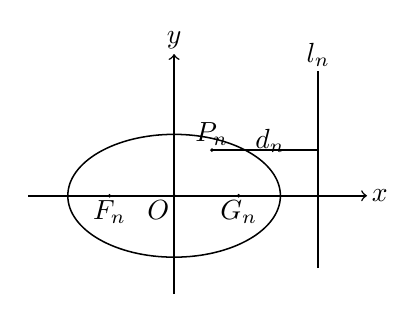
\begin{tikzpicture}[x=1cm,y=1cm,line width=0.55pt,every node/.style={inner sep=1.5pt}]
 % Ellipse, coordinate axes, right directrix l_n, point P_n, foci and horizontal distance d_n.
 \draw (0,0) ellipse (1.35 and 0.78);
 \draw[->] (-1.85,0)--(2.45,0) node[right] {$x$};
 \draw[->] (0,-1.25)--(0,1.8) node[above] {$y$};
 \draw (1.83,-0.92)--(1.83,1.58) node[above] {$l_n$};
 \coordinate (Pn) at (0.48,0.58); \coordinate (Fn) at (-0.82,0); \coordinate (Gn) at (0.82,0);
 \fill (Pn) circle (0.025) node[above] {$P_n$};
 \fill (Fn) circle (0.025) node[below] {$F_n$};
 \fill (Gn) circle (0.025) node[below] {$G_n$};
 \fill (0,0) circle (0.025) node[below left] {$O$};
 \draw (Pn)--(1.83,0.58);
 \node at (1.22,0.70) {$d_n$};
\end{tikzpicture}
